\documentclass[11pt]{article}
\usepackage[margin=1.15in]{geometry}
\usepackage{amsmath,amssymb,amsthm}
\usepackage{booktabs}
\usepackage{graphicx}
\usepackage{microtype}
\usepackage[authoryear,round]{natbib}
\usepackage[colorlinks=true,linkcolor=black,citecolor=black,urlcolor=black]{hyperref}
\usepackage{setspace}
\onehalfspacing

\newtheorem{proposition}{Proposition}
\theoremstyle{definition}
\newtheorem{definition}{Definition}
\newcommand{\E}{\mathbb{E}}

\title{Which Trials Count\\[4pt]
\large Inclusion Rules, Influence, and the Reproducibility of a Pooled Estimate}
\author{Flyxion\\Independent Researcher}
\date{October 2026}

\begin{document}
\maketitle

\begin{abstract}
\noindent
Three meta-analyses of antidepressant treatment for depression in children and adolescents reached different conclusions about fluoxetine, and a recent news report attributes the disagreement to one small trial that two of the analyses included and the third excluded for an unrelated reason. This essay uses that episode to examine how a pooled estimate depends on the set of trials that enter it. An inclusion rule written to define relevance, such as a comparator class, can retain or remove a flawed trial by accident, so that agreement or disagreement among reviews can be an artefact of scope and not evidence about the treatment. How far a single trial moves a network estimate depends on the precision of the direct evidence, and a small network computation shows shifts from $0.17$ to $2.0$ points on a depression scale for the same aberrant trial as the direct evidence weakens. Standard inverse-variance weights down-weight an implausibly large standardized effect only mildly. A conclusion phrased as statistical significance can flip under a modest shift while a conclusion phrased against a pre-specified equivalence range need not, which the arithmetic for the most recent review's fluoxetine estimate makes concrete. The essay closes with reporting practices that make a review's dependence on any one trial visible. The analysis concerns method; it does not evaluate the clinical use of any drug, and the trial in question is discussed only through what has been reported about it by others.
\end{abstract}

\section{Three analyses, one trial}

Several clinical guidelines recommend fluoxetine as a first treatment for depression in children and adolescents, citing a 2016 network meta-analysis and a 2020 follow-up. A 2021 Cochrane network meta-analysis \citep{hetrick2021} reached a more guarded conclusion, finding only small effects. A news report \citep{vannoorden2026} summarizes a 2026 analysis \citep{lyus2026} as finding that the disagreement among the three reflects whether a single trial of 40 children, published in 2006, was included. According to the report, that trial showed a very large advantage of fluoxetine over nortriptyline, a tricyclic antidepressant; re-running the earlier meta-analyses without it removed fluoxetine's outsized benefit; and the 2021 review omitted the trial because it excluded comparisons involving the drug class that nortriptyline belongs to. The report also describes concerns about the trial's reported data, including a pattern in which every participant's score appeared to change by a similar amount, and the absence of a description of ethics approval.

The 2026 analysis was not available for this essay, and what follows about it rests on the news report. The 2021 review was read directly. Its scope statement defines new-generation antidepressants as those that ``do not include older formulations (tricyclic antidepressants or monoamine oxidase inhibitors),'' which is consistent with the report's account of why a nortriptyline comparison fell outside it.

The episode is useful independently of how the clinical question is resolved, because it exhibits a general feature of evidence synthesis: the output depends on a set of inputs defined by rules whose purpose is not the quality of the inputs.

\section{Inclusion as an argument of the estimate}

Write $\hat\theta(S)$ for a pooled estimate computed from the set $S$ of included trials, and define the influence of trial $j$ as $\Delta_j=\hat\theta(S)-\hat\theta(S\setminus\{j\})$. Three rules decide $S$ in practice. A scope rule defines relevance (population, treatments, comparators, outcomes). A quality rule excludes trials judged at high risk of bias or untrustworthy. A data rule excludes trials that do not report usable outcomes. A given trial can be retained or removed by any of them, and nothing makes the three rules agree.

In the reported episode the removal was by a scope rule, written to keep a review about newer drugs, and its effect on the pooled estimate for fluoxetine was incidental. Two consequences follow.

\paragraph{Robustness by accident is not robustness.} The 2021 conclusion did not rest on the flawed trial, but its authors did not know that, in the sense that no analysis of theirs tested it. The result is robust to that trial in the way a house is robust to a flood that bypassed it.

\paragraph{Agreement among reviews counts less than it appears to.} If two analyses share a trial that carries the result, a third analysis that omits it is not a rival confirmation of one side, it is a test of whether the shared trial matters. The effective number of independent confirmations of a finding is reduced by overlap in the trial sets, and in a field with only a few dozen trials, overlap is large. A tally of ``two of three reviews support'' counts the shared input twice.

\section{How far one trial moves a network estimate}

The trial in question compared fluoxetine (F) with nortriptyline (N). The estimate that matters for guidelines is fluoxetine against placebo (P). A trial on the F--N edge enters the F--P estimate only through the network: it informs $\theta_F-\theta_N$, which combines with evidence on $\theta_N$ to bear on $\theta_F$. How much it moves the F--P estimate depends on how much other evidence pins $\theta_F$ down.

A small fixed-effect network shows the dependence. Let the direct F--P evidence be an estimate of $-2.8$ scale points (the order of magnitude of the 2021 review's fluoxetine estimate, used here only as a number) with standard error $s$; the direct N--P evidence be $-2.0$ with standard error $2.0$; and a single F--N trial report a difference $-d$ with standard error $2.5$, where the value consistent with the other two is $-0.8$. The network estimate of $\theta_F$ is the weighted least-squares solution. Table~\ref{tab:shift} gives the shift in the F--P estimate when the F--N trial reports $-12$, an implausibly large difference, and Table~\ref{tab:split} gives the F--N inconsistency test (direct against indirect) when $s=0.65$.

\begin{table}[h]
\centering
\caption{Shift in the network estimate of fluoxetine versus placebo (scale points) when one fluoxetine versus nortriptyline trial reports a difference of $-12$ instead of the consistent $-0.8$, by the standard error $s$ of the direct fluoxetine versus placebo evidence.}
\label{tab:shift}
\begin{tabular}{rcccc}
\toprule
direct standard error $s$ & 0.40 & 0.65 & 1.00 & 1.50 \\
\midrule
shift in the F--P estimate & $-0.17$ & $-0.44$ & $-1.00$ & $-2.02$ \\
\bottomrule
\end{tabular}
\end{table}

\begin{table}[h]
\centering
\caption{The same network with $s=0.65$. Network estimate of fluoxetine versus placebo and the $P$ value of a direct-versus-indirect inconsistency test for the F--N edge, by the difference reported in the single F--N trial.}
\label{tab:split}
\begin{tabular}{rccccc}
\toprule
reported F--N difference & $-0.8$ & $-3$ & $-5$ & $-8$ & $-12$ \\
\midrule
network F--P estimate & $-2.80$ & $-2.89$ & $-2.97$ & $-3.09$ & $-3.24$ \\
inconsistency $P$ & 1.00 & 0.50 & 0.20 & 0.028 & 0.0006 \\
\bottomrule
\end{tabular}
\end{table}

An isolated trial on a different edge moves an estimate that is directly well measured by a fraction of a point, and moves a poorly measured one by about two points, which is as large as the estimate itself. Whether a single trial can change a conclusion therefore is not decided by argument. It depends on the network's geometry, and it can only be answered by computing the influence. Where a loop exists the inconsistency test flags the aberrant edge, but a test needs direct evidence on the edge, and the 2021 review itself notes for some comparisons that possible inconsistency was inconclusive because direct evidence was limited. A single trial on an edge by itself is a situation in which such a test has little power.

The calculation is a fixed-effect toy. A random-effects model treats a discrepant trial as heterogeneity, which widens intervals but still lets the trial move the centre. No network, number or estimate here belongs to any of the three reviews, and the toy does not reproduce the reported reversal. Its purpose is to show that the reported reversal is possible for particular networks and not for others.

\section{What the weights do with an implausible trial}

An inverse-variance meta-analysis weights each trial by the reciprocal of the variance computed from its reported summary statistics. When a trial reports an implausibly small spread, for example because scores changed by almost the same amount in every participant, the standardized effect, the mean difference divided by the standard deviation, becomes very large. The variance of a standardized difference $d$ with $n$ per arm is approximately $2/n+d^2/(4n)$, so the weight $1/\mathrm{var}$ falls as $d$ grows, but slowly. Table~\ref{tab:smd} takes a raw difference of $8$ scale points and $20$ participants per arm, and varies the standard deviation of change.

\begin{table}[h]
\centering
\caption{Standardized effect and inverse-variance weight for a fixed raw difference of 8 points, $n=20$ per arm, as the reported standard deviation of change shrinks. The last row is a conventional effect of $d=0.3$.}
\label{tab:smd}
\begin{tabular}{rccc}
\toprule
reported SD of change & $d$ & standard error & weight \\
\midrule
12 & 0.67 & 0.32 & 9.5 \\
6 & 1.33 & 0.35 & 8.2 \\
3 & 2.67 & 0.43 & 5.3 \\
\midrule
(conventional effect) & 0.30 & 0.32 & 9.9 \\
\bottomrule
\end{tabular}
\end{table}

A report with an effect nine times the conventional size receives about half the weight of a conventional one. The formula treats the reported variability as true. It has no mechanism for suspecting that variability reported as small may signal a problem with the data and not an extremely consistent effect, and a trial whose numbers are wrong for non-sampling reasons violates the assumption that errors are independent sampling noise. Weighting cannot detect this. The figures in the table are generic arithmetic, and the actual numbers of the trial in question were not available for this essay.

\begin{figure}[h]
\centering
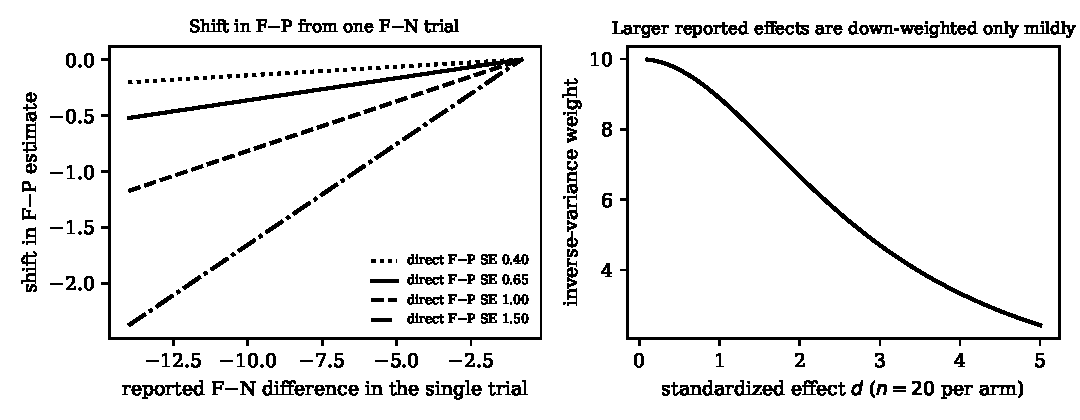
\includegraphics[width=\textwidth]{fig_nma.pdf}
\caption{Left: shift in the network estimate of F versus P as the single F versus N trial reports an increasingly large difference, for four precisions of the direct F versus P evidence. Right: inverse-variance weight of a standardized effect $d$ at $n=20$ per arm.}
\label{fig:nma}
\end{figure}

\section{Significance flips; equivalence ranges do not}

The 2021 review pre-specified an equivalence range of $-5$ to $5$ points on the clinician-rated scale and described an effect as ``small and unimportant'' if its estimate fell inside it. For fluoxetine against placebo it reported a mean difference of $-2.84$ (95\% interval $-4.12$ to $-1.56$) with moderate-certainty evidence, so that fluoxetine ``probably'' produces a small and unimportant reduction, and it concluded that fluoxetine, along with sertraline, escitalopram and duloxetine, could be considered as a first option for some individuals in some circumstances.

The arithmetic of robustness for these two statements differs. The interval stays inside the equivalence range unless the estimate moves by more than $5-4.12=0.88$ points towards a larger benefit, and it is about $1.56$ points from excluding zero in the other direction. A conclusion of the form ``statistically significant against placebo'' is crossed by a shift of $1.56$ points, while one of the form ``within the equivalence range'' is crossed by $0.88$ in the other direction. The two lines are at different distances ($0.88$ and $1.56$ points) and they answer different questions: one asks whether any effect can be distinguished from zero, the other whether it is large enough to matter. A literature that reports only the first will show reversals whenever a shift is large enough to cross a boundary that sits close to the estimate. The reported reversal, from a significant advantage to no advantage, is a reversal of that kind. How near the earlier analyses' intervals were to the boundary is not reported in the news item, and the question of whether the estimate moved by one point or by several is one that the 2026 analysis answers and that this essay could not check.

The review's own wording shows the alternative. It attached a certainty grade and an importance label to each estimate, and those two ideas carry across moderate shifts in a way that significance does not. The note that the 2016 and 2020 analyses placed ``very low'' confidence on the fluoxetine finding, which the news report attributes to one of their authors, makes the same point from the other side: the information was present, and the question is why it did not reach the guidelines.

\section{From estimate to recommendation}

A recommendation cites an estimate, and the estimate carries qualifiers that the recommendation seldom repeats. The news item reports that a prescribing handbook cites the 2020 analysis for fluoxetine having the strongest current evidence of efficacy, and that its editor expects the next edition to acknowledge that the evidence is open to different interpretations. The chain from trial to estimate to certainty grade to guideline sentence loses information at each step, and the loss is systematic: direction and significance survive, interval width and certainty do not.

There is also a part of the question that no re-analysis settles. A small average improvement may be worth having for some patients and not for others, and, as the news item quotes, there is no consensus on what magnitude counts as clinically meaningful. The 2021 review makes this explicit by stating that averages conceal individuals who may respond more. A correction to the evidence base changes the estimate. Whether the corrected estimate justifies a recommendation is a judgement about values and risks, and it is separate from the statistical question.

\section{Reporting that makes dependence visible}

\begin{enumerate}
\item \textbf{Influence table.} Every network meta-analysis can report the estimate, the interval and the equivalence-range class for each key comparison with each trial left out in turn. The computation is cheap and removes the need to argue about whether a trial matters.
\item \textbf{Scope multiverse.} Re-running the analysis under the plausible alternative scope rules, such as including or excluding a comparator class, shows when a conclusion is a feature of the rule.
\item \textbf{Report exclusions by reason.} List the studies excluded for scope and for quality separately, and flag any excluded study that would have been influential if included, since scope exclusions are the ones that hide flawed data.
\item \textbf{Pre-specified trustworthiness screening.} Apply the screening protocol to all included trials, including the large-effect outliers, and report results with and without suspect trials.
\item \textbf{Cite estimates with their qualifiers.} A guideline sentence should cite the estimate, interval, equivalence class and certainty grade together, and name the analysis version.
\item \textbf{Count independence.} When several reviews agree, report the overlap in trial sets and treat shared trials as one source.
\end{enumerate}

\section{Conclusion}

A pooled estimate is a function of which trials count, and the rules that decide are written for other purposes. In the reported episode a scope rule kept one review clear of a trial that two others included, and the divergence was read as disagreement about the drug. The size of such an effect depends on the network, on the weights, and on how close the conclusion sits to a threshold, all of which can be computed, and the first remedy is to compute them and report them. The second is to cite the estimate together with the qualifiers that determine what it supports.

\begin{thebibliography}{9}
\bibitem[Hetrick et al.(2021)]{hetrick2021} Hetrick, S.~E., McKenzie, J.~E., Bailey, A.~P., Sharma, V., Moller, C.~I., Badcock, P.~B., Cox, G.~R., Merry, S.~N., Meader, N. (2021). New generation antidepressants for depression in children and adolescents: a network meta-analysis. \emph{Cochrane Database of Systematic Reviews}, Issue 5, Art. No. CD013674. doi:10.1002/14651858.CD013674.pub2.
\bibitem[Lyus et al.(2026)]{lyus2026} Lyus, R., Naudet, F., van Valkenhoef, G., Pl\"oderl, M. (2026). \emph{Cochrane Evidence Synthesis and Methods} 4, e70108. Cited as reported in \citet{vannoorden2026}; not read for this essay.
\bibitem[Van Noorden(2026)]{vannoorden2026} Van Noorden, R. (2026). Prozac use for childhood depression skewed by single flawed medical trial. \emph{Nature} (news), 2 October 2026. doi:10.1038/d41586-026-02769-x.
\end{thebibliography}

\end{document}
